\section*{Введение}
\addcontentsline{toc}{section}{Введение}

Датчики угла поворота (ДУП) --- устройства, предназначенные для преобразования угла поворота вращающегося объекта (вала) в электрические сигналы, позволяющие определить угол его поворота. Датчики угла поворота имеют множество применений. Они широко применяются в промышленности (в частности в сервоприводах), в роботостроении, в автомобилестроении (например для определения угла поворота рулевого колеса), в компьютерной технике (для определения угла поворота колеса компьютерной мыши) и т.п. \cite{wiki:rotary} Также энкодеры используются в станках ЧПУ для точного позиционирования \cite{educ:encoders}.

Типичный энкодер изображен на рисунке \ref{fig:encoder}. Внешне он похож на потенциометр с тем отличием, что крутить его можно бесконечно в любую сторону.

\begin{figure}[ht]
    \subfloat[]{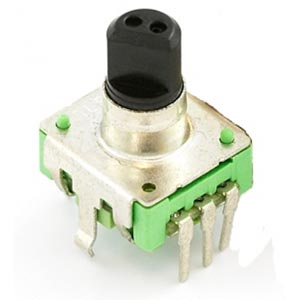
\includegraphics[width=.4\linewidth]{Figures/encoder.png}}
    \subfloat[]{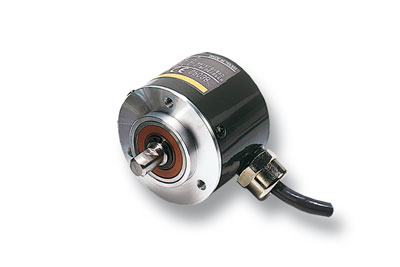
\includegraphics[width=.6\linewidth]{Figures/indenc.png}}
    \caption{Типичный энкодер (a) бытовой; (б) промышленный}
    \label{fig:encoder}
\end{figure}

В основе работы энкодера лежит фотоэлектрический бесконтактный датчик, работающий на просвет и считывающий информацию со специальным образом перфорированного колеса. Благодаря большому количеству отверстий (до 10000 на оборот) каждая дуга углового перемещения может быть разделена на мельчайшие отрезки величиной менее миллиметра \cite{rusauto:enc}.

Информация в виде последовательности импульсов поступает на контроллер, анализирующий сигналы, поступающие с энкодера и преобразовывает эту последовательность в данные о положении вала или количество оборотов.

ДУПы подразделяются по способу выдачи информации на \textbf{накапливающие} (инкрементные) и \textbf{абсолютные} (позиционные), по принципу действия на \textbf{оптические}, \textbf{резистивные}, \textbf{магнитные}, \textbf{индуктивные}, \textbf{механические} \cite{wiki:rotary}. В докладе мы рассматриваем \textbf{оптические} преобразователи, работающие с датчиками \textbf{накапливающего} типа, а также \textbf{абсолютные} (кодирующие) преобразователи перемещений.

Накапливающие ДУПы на выходе формируют импульсы, по которым принимающее устройство определяет текущее положение вала путем подсчета числа импульсов счётчиком. Сразу же после включения накапливающего ДУПа положение вала неизвестно. Для привязки системы отсчета к началу отсчёта инкрементые датчики имеют нулевые (референтные) метки, через которые нужно пройти после включения оборудования. К недостаткам такого типа датчиков угла положения также относится то, что невозможно определить пропуск импульсов от ДУПа по каким-либо причинам. Это приводит к накоплению ошибки определения угла поворота вала до тех пор, пока не будет пройдена нуль-метка. Для определения направления вращения применяются два измерительных канала (``синусный'' и ``косинусный''), в которых идентичные последовательности импульсов (меандры) сдвинуты на $90^{\circ}$ (парафазные импульсы) относительно друг друга (рисунок \ref{fig:meandr}).

\begin{figure}[ht]
    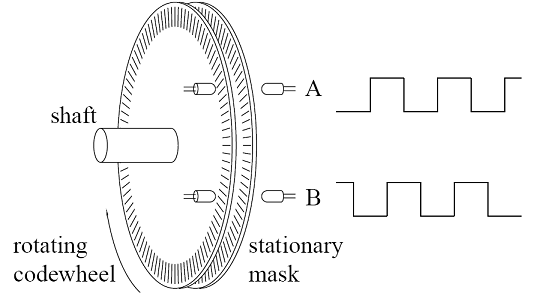
\includegraphics[width=1\linewidth]{Figures/meandr.png}
    \caption{Сигналы с выхода энкодера\label{fig:meandr}}
\end{figure}

\section{Устройство энкодера накапливающего типа}

У нас имеется диск с двумя дорожками, на которых есть светлые и темные участки (рисунок \ref{fig:disk}).

\begin{figure}[ht]
    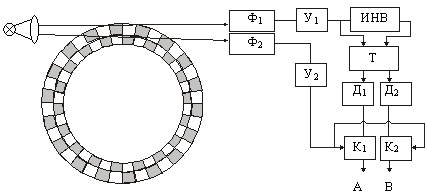
\includegraphics[width=1\linewidth]{Figures/disk.png}
    \caption{Диск оптического преобразователя\label{fig:disk}}
\end{figure}

Условные обозначения:

\begin{itemize}
    \item $\textup{Ф}_1$ и $\textup{Ф}_2$ --- фотоприемники;
    \item $\textup{Д}_1$ и $\textup{Д}_2$ --- дифференцирующие элементы (одновибраторы);
    \item $\textup{У}_1$ и $\textup{У}_2$ --- усилители;
    \item $\textup{К}_1$ и $\textup{К}_2$ --- ключи;
    \item Т --- триггер.
\end{itemize}

Счетчик при движении вправо --- накапливает, влево --- сбрасывает (рисунок \ref{fig:reverse}). Вправо --- по шине A, влево --- по шине B. Возникающие при этом сигналы на элементах схемы приведены на рисунке \ref{fig:complex}.

\begin{figure}[ht]
    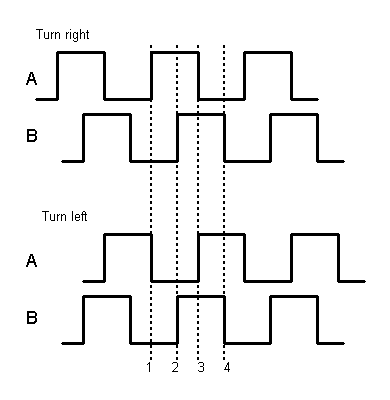
\includegraphics[width=0.6\linewidth]{Figures/reverse.png}
    \caption{Направление вращения\label{fig:reverse}}
\end{figure}

\begin{figure}[ht]
    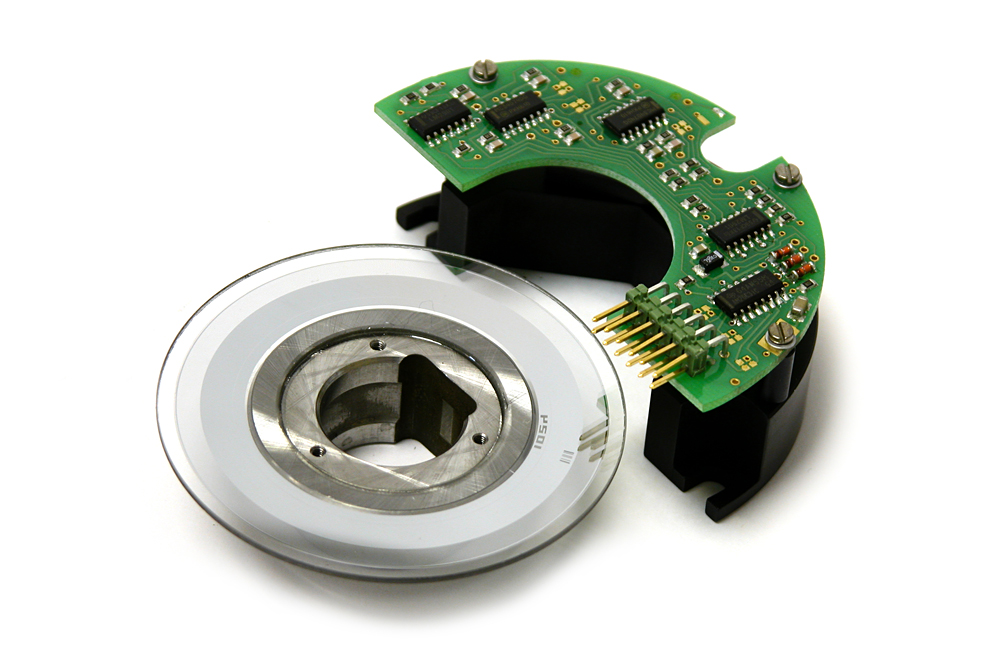
\includegraphics[width=.4\linewidth]{Figures/splitenc.png}
    \caption{Фотоэлектрический энкодер}
    \label{fig:splitenc}
\end{figure}

\begin{figure}[ht]
    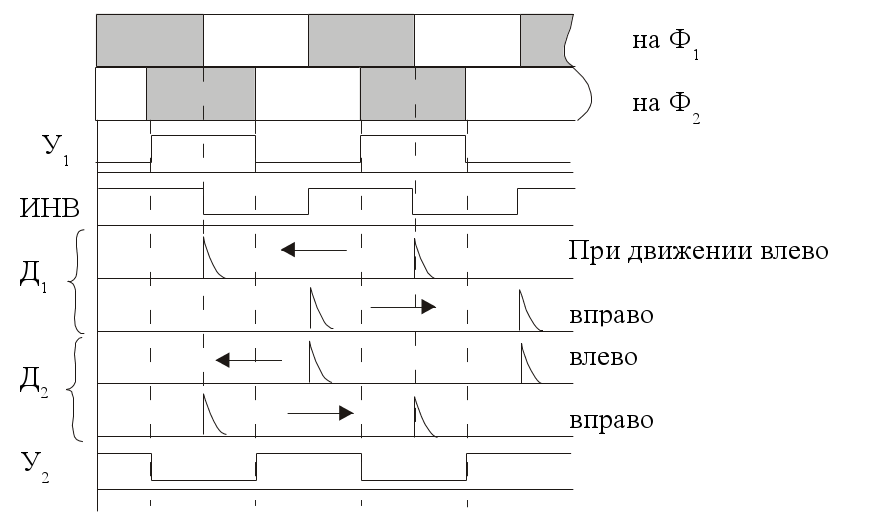
\includegraphics[width=1\linewidth]{Figures/complex.png}
    \caption{Сигналы на элементах\label{fig:complex}}
\end{figure}

Основным рабочим параметром датчика является количество импульсов за один оборот. Для вычисления угловой скорости объекта процессор в тахометре выполняет дифференцирование количества импульсов во времени, таким образом показывая сразу величину скорости, то есть число оборотов в минуту. Наличие парафазных импульсов позволяет определять направление вращения. Имеется также цифровой выход нулевой метки, который позволяет всегда рассчитать абсолютное положение вала \cite{epromauto:enc}. Внутренний вид микросхем, отвечающих за расчеты, отображен на рисунке \ref{fig:splitenc}.

\section{Устройство энкодера абсолютного типа}

Эти энкодеры являются более совершенными. В таких преобразователях каждому значению угла поворота соответствует своя кодовая комбинация, соответственно они не требуют привязки системы отсчёта к какому-либо нулевому положению.

Основная характеристика таких энкодеров --- число шагов, то есть уникальных кодов на оборот и количество таких оборотов, при этом не требуется первичной установки и инициализации датчика. Поэтому абсолютные энкодеры не теряют свою позицию при исчезновении напряжения \cite{epromauto:enc}.

Абсолютный энкодер относится к типу энкодеров, который выполняет уникальный код для каждой позиции вала. В отличие от инкрементного энкодера, счетчик импульсов не нужен,т.к. угол поворота всегда известен. Абсолютный энкодер формирует сигнал как во время вращения, так и в режиме покоя. Диск абсолютного энкодера отличается от диска пошагового энкодера, так как имеет несколько концентрических дорожек. Каждой дорожкой формируется уникальный двоичный код для конкретной позиции вала (рисунок \ref{fig:code}).

\begin{figure}[ht]
    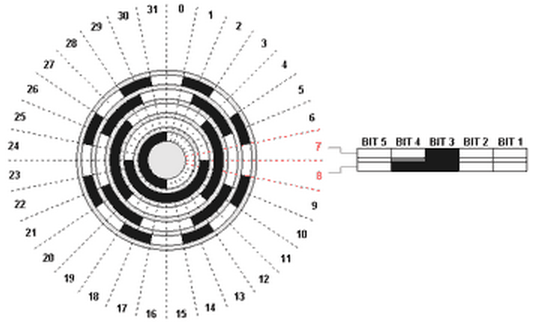
\includegraphics[width=.7\linewidth]{Figures/code.png}
    \caption{Кодовый диск абсолютного энкодера}
    \label{fig:code}
\end{figure}

Простейший пример такого энкодера --- энкодер с тремя дорожками (рисунок \ref{fig:3contacts}) \cite{wiki:enrotary}.

\begin{figure}[ht]
    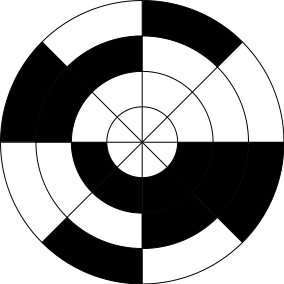
\includegraphics[width=0.3\linewidth]{Figures/3contacts.png}
    \caption{Двоичный код трехдорожкового энкодера\label{fig:3contacts}}
\end{figure}

Количество возможных позиций (дискретность) энкодера определяется как $2^n$, где n --- число дорожек, что в данном случае представляет $2^3 = 8$ позиций. Представим их в виде таблицы \ref{tab:3contacts}.

\begin{longtable}[c]{|c|c|c|c|c|}
    \caption{Стандартная двоичная кодировка\label{tab:3contacts}}\\
    \hline
    \multirow{2}{*}{\textbf{Сектор}} & \multicolumn{3}{|c|}{\textbf{Номер дорожки}} & \multirow{2}{*}{\textbf{Диапазон}}\\
    \cline{2-4}
    & \textbf{1} & \textbf{2} & \textbf{3} &\\
    \hline
    \endfirsthead
    \hline
    \textbf{Сектор} & \textbf{Дорожка 1} & \textbf{Дорожка 2} & \textbf{Дорожка 3} & \textbf{Диапазон}\\
    \hline
    \endhead
    0 & off & off & off & $0^{\circ}$ -- $45^{\circ}$\\
    \hline
    1 & off & off & \cellcolor{green!20}ON & $45^{\circ}$ -- $90^{\circ}$\\
    \hline
    2 & off & \cellcolor{green!20}ON & off & $90^{\circ}$ -- $135^{\circ}$\\
    \hline
    3 & off & \cellcolor{green!20}ON & \cellcolor{green!20}ON & $135^{\circ}$ -- $180^{\circ}$\\
    \hline
    4 & \cellcolor{green!20}ON & off & off & $180^{\circ}$ -- $225^{\circ}$\\
    \hline
    5 & \cellcolor{green!20}ON & off & \cellcolor{green!20}ON & $225^{\circ}$ -- $270^{\circ}$\\
    \hline
    6 & \cellcolor{green!20}ON & \cellcolor{green!20}ON & off & $270^{\circ}$ -- $315^{\circ}$\\
    \hline
    7 & \cellcolor{green!20}ON & \cellcolor{green!20}ON & \cellcolor{green!20}ON & $315^{\circ}$ -- $360^{\circ}$\\
    \hline
\end{longtable}

Во время вращения диска дорожки производят обыкновенный двоичный код, однако в этом самом коде кроется огромный недостаток. Предположим, наш диск дошел до отметки $179.9^{\circ}$ и переходит к отметке $180.1^{\circ}$ (из третьего сектора в четвертый). В некоторый момент, соответственно таблице \ref{tab:3contacts}, дорожки переключатся из состояния \textbf{off-on-on} в состояние \textbf{on-off-off}. Однако из-за наличия помех и неравномерного расположения дорожек состояния переключатся в неопределенном порядке: например --- сначала третий, потом первый и затем второй. В результате мы получим подобную картину:

\clearpage %KOSTYL

\begin{verbatim}
off-on-on
off-on-off
on-on-off
on-off-off
\end{verbatim}

В итоге, при переключении сложится неопределенное состояние и нельзя будет однозначно утверждать какой угол поворота у вала в текущий момент. Данную проблему решает использование циклических кодов, в которых ошибка считывания может быть только в самом младшем разряде. Наиболее распространенные типы выходов сигнала --- это код Грея, параллельный код, интерфейсы Profibus-DP, CANopen, DeviceNet, SSI, LWL и другие \cite{epromauto:enc}.

\section{Код Грея}

Код Грея --- это система двоичного исчисления устроенная таким образом, чтобы любые два ближайшие кода отличались лишь одним битом. Для примера, рассмотрим трехдорожковую систему приведенную выше (таблица \ref{tab:gray}).

\begin{longtable}[c]{|c|c|c|c|c|}
    \caption{Кодировка Грея\label{tab:gray}}\\
    \hline
    \multirow{2}{*}{\textbf{Сектор}} & \multicolumn{3}{|c|}{\textbf{Номер дорожки}} & \multirow{2}{*}{\textbf{Диапазон}}\\
    \cline{2-4}
    & \textbf{1} & \textbf{2} & \textbf{3} &\\
    \hline
    \endfirsthead
    \hline
    \textbf{Сектор} & \textbf{Дорожка 1} & \textbf{Дорожка 2} & \textbf{Дорожка 3} & \textbf{Диапазон}\\
    \hline
    \endhead
    0 & off & off & off & $0^{\circ}$ -- $45^{\circ}$\\
    \hline
    1 & off & off & \cellcolor{green!20}ON & $45^{\circ}$ -- $90^{\circ}$\\
    \hline
    2 & off & \cellcolor{green!20}ON & \cellcolor{green!20}ON & $90^{\circ}$ -- $135^{\circ}$\\
    \hline
    3 & off & \cellcolor{green!20}ON & off & $135^{\circ}$ -- $180^{\circ}$\\
    \hline
    4 & \cellcolor{green!20}ON & \cellcolor{green!20}ON & off & $180^{\circ}$ -- $225^{\circ}$\\
    \hline
    5 & \cellcolor{green!20}ON & \cellcolor{green!20}ON & \cellcolor{green!20}ON & $225^{\circ}$ -- $270^{\circ}$\\
    \hline
    6 & \cellcolor{green!20}ON & off & \cellcolor{green!20}ON & $270^{\circ}$ -- $315^{\circ}$\\
    \hline
    7 & \cellcolor{green!20}ON & off & off & $315^{\circ}$ -- $360^{\circ}$\\
    \hline
\end{longtable}

Здесь при переходе из сектора 3 в сектор 4 изменяется лишь один бит, что устраняет возможность появления на дорожках очередности неверных кодов.

Чтобы найти циклический код десятичного числа, необходимо найти его двоичный эквивалент, а затем перевести его в циклический по правилу. Если в старшем разряде двоичного кода стоит ноль, то в данном разряде циклического кода цифра не меняется, а если единица --- меняется на обратную (таблица \ref{tab:bintogray}). Маски двоичного и циклического кодов представлены на рисунке \ref{fig:bincycle}.

\begin{longtable}[c]{|c|c|c|}
    \caption{Перевод из двоичного кода в код грея\label{tab:bintogray}}\\
    \hline
    \textbf{Десятичное число} & \textbf{Двоичный код} & \textbf{Код Грея}\\
    \hline
    \endfirsthead
    \hline
    \textbf{Десятичное число} & \textbf{Двоичный код} & \textbf{Код Грея}\\
    \hline
    \endhead
    0 & 0000 & 0000\\
    \hline
    1 & 0001 & 0001\\
    \hline
    2 & 0010 & 0011\\
    \hline
    3 & 0011 & 0010\\
    \hline
    4 & 0100 & 0110\\
    \hline
    5 & 0101 & 0111\\
    \hline
\end{longtable}

\begin{figure}[ht]
    \subfloat[]{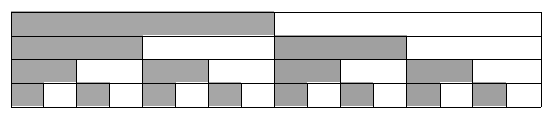
\includegraphics[width=.5\linewidth]{Figures/binarymask.png}}
    \subfloat[]{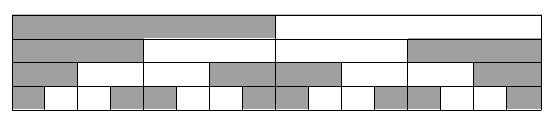
\includegraphics[width=.5\linewidth]{Figures/cyclemask.png}}
    \caption{Маски (а) бинарного кода; (б) циклического кода\label{fig:bincycle}}
\end{figure}

Обратный переход от кода Грея к двоичному осуществляется по правилам:

\begin{enumerate}
    \item Все цифры в старших разрядах до первой единицы в двоичном коде такие же, как и в коде Грея.
    \item В остальных разрядах цифры совпадают, если перед данным разрядом (со стороны старших) было четное число единиц.
    \item Если число единиц в коде Грея было нечетным, то данная цифра в двоичном коде заменяется на обратную.
\end{enumerate}

\paragraph*{Пример:} 1100101 $\rightarrow$ 1000110.

На вращающемся диске нанесен код Грея, который преобразуется в двоичный код для дальнейшей работы. Работа преобразователя представлена на рисунках \ref{fig:commonchanger}, \ref{fig:changer} и \ref{fig:complexchanger}.

\begin{figure}[ht]
    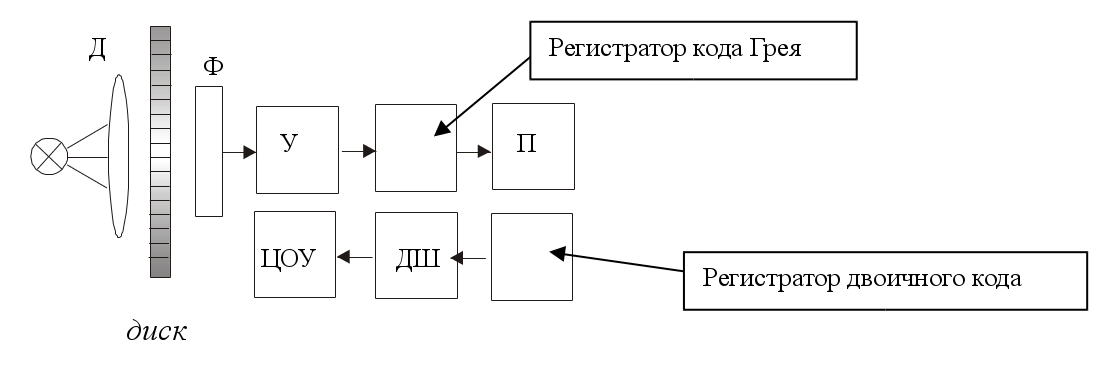
\includegraphics[width=1\linewidth]{Figures/commonchanger.png}
    \caption{Схема преобразователя\label{fig:commonchanger}}
\end{figure}

Условные обозначения:

\begin{itemize}
    \item Д --- диафрагма;
    \item Ф --- фотоприёмник;
    \item П --- преобразователь;
    \item ДШ --- дешифратор;
    \item ЦОУ --- цифровое отсчетное устройство.
\end{itemize}

\begin{figure}[ht]
    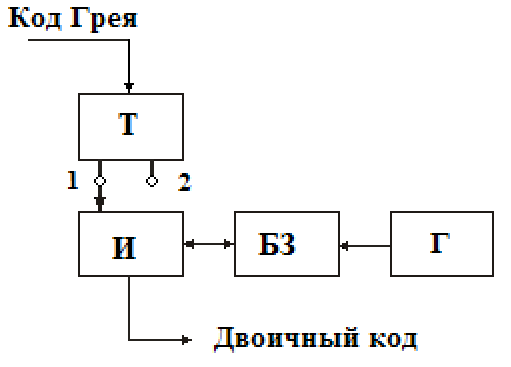
\includegraphics[width=0.5\linewidth]{Figures/changer.png}
    \caption{Работа преобразователя П}
    \label{fig:changer}
\end{figure}

Условные обозначения:

\begin{itemize}
    \item Т --- триггер;
    \item 1 --- сигнал с выхода триггера;
    \item 2 --- для получения инверсного сигнала;
    \item И --- логический элемент ``И'';
    \item Г --- импульсный генератор;
    \item БЗ --- блок задержки.
\end{itemize}

\begin{figure}[ht]
    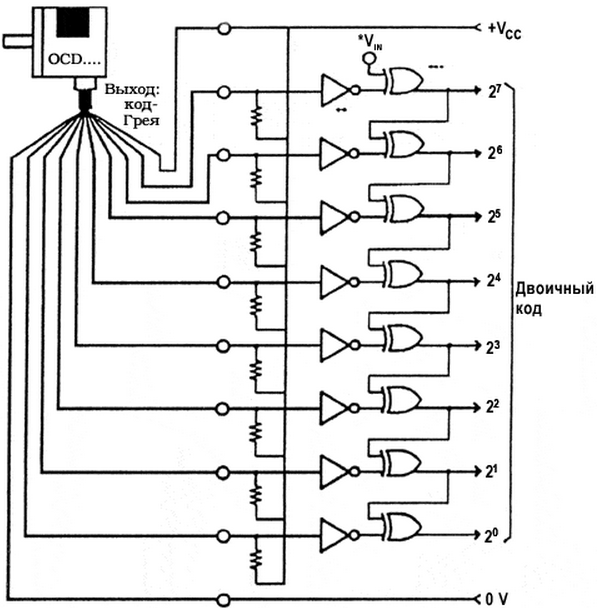
\includegraphics[width=1\linewidth]{Figures/complexchanger.png}
    \caption{Схема для преобразования Кода Грея в двоичный код}
    \label{fig:complexchanger}
\end{figure}

На триггер Т со счетным входом подаются импульсы кода Грея, начиная со старшего разряда. С выхода 1 триггера импульсы подаются на первый вход логического элемента И. На второй вход И через БЗ синхронно с импульсами кода Грея подаются импульсы от тактового генератора Г. БЗ задерживает импульсы Г, чтобы триггер успел переброситься из устойчивого состояния в другое.

\section{Применение энкодеров}

Энкодеры применяются не только в разных системах автоматизации, станках ЧПУ и роботостроении, но также могут и применяться для повседневных задач обыкновенного пользователя, например для регулирования громкости интернет-радиостанции или просто домашнего медиацентра.

Рассмотрим простой энкодер COM-09117, используемых для повседневных задач оптимизации. Он имеет 3 ноги, подключаемые соответственно к земле и к двум GPIO (General-Purpose Input/Output) ногам (рисунок \ref{fig:pins}). С выходов A и B поступают сигналы в соответствии с рисунком \ref{fig:signals} \cite{bob:rpirotary}.

\begin{figure}[ht]
    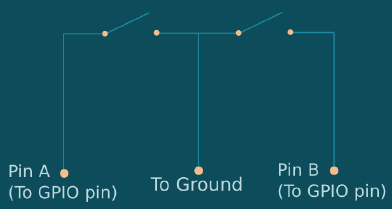
\includegraphics[width=.5\linewidth]{Figures/pins.png}
    \caption{Распиновка энкодера}
    \label{fig:pins}
\end{figure}

\begin{figure}[ht]
    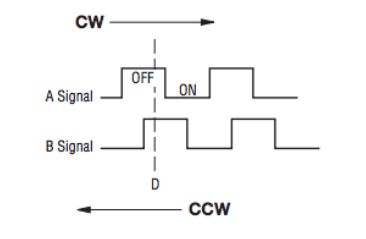
\includegraphics[width=.5\linewidth]{Figures/signals.png}
    \caption{Сигналы с выходов A и B}
    \label{fig:signals}
\end{figure}

Исходя из этих сигналов необходимо определить в какую сторону вращается энкодер. Это можно сделать используя побитовую логическую коньюнкцию (XOR-значение) выходов A и B (таблица \ref{tab:xor}).

\begin{longtable}[c]{|c|c|c|c|c|}
    \caption{Последовательность энкодера по часовой стрелке}
    \label{tab:xor}\\
    \hline
    \textbf{Последовательность} & \textbf{A} & \textbf{B} & \textbf{$A\land B$ (C)} & \textbf{Значение}\\
    \hline
    \endfirsthead
    \hline
    \textbf{Последовательность} & \textbf{A} & \textbf{B} & \textbf{$A^B$ (C)} & \textbf{Значение}\\
    \hline
    \endhead
        0 & 0 & 0 & 0 & 0\\
        \hline
        1 & 1 & 0 & 1 & 5\\
        \hline
        2 & 1 & 1 & 0 & 6\\
        \hline
        3 & 0 & 1 & 1 & 3\\
        \hline
\end{longtable}

Теперь, когда у нас есть битовая последовательность поворота энкодера по часовой стрелке, нам остается узнать в какую, собственно, сторону он был повернут. Это достигается определением разницы между новым и предыдущим значениями. На языке программирования python этого можно достичь следующим кодом:

\begin{verbatim}
    delta = (new_state - last_state) % 4
\end{verbatim}

Здесь \%4 --- операция, возвращающая остаток от деления на 4. Соответственно, получаем определенную интерпретацию в зависимости от \textbf{delta} (таблица \ref{tab:delta}).

\begin{longtable}[c]{|c|c|}
    \caption{Интерпретация событий в зависимости от текущего значения delta}
    \label{tab:delta}\\
    \hline
    \textbf{delta} & \textbf{Соответствие}\\
    \hline
    \endfirsthead
    \hline
    \textbf{delta} & \textbf{Соответствие}\\
    \hline
    \endhead
        0 & Нет изменений\\
        \hline
        1 & Один шаг по часовой стрелке\\
        \hline
        2 & Два шага по часовой стрелке или против часовой стрелки\\
        \hline
        3 & Один шаг против часовой стрелки\\
        \hline
\end{longtable}

Используя эти данные, а также подключив энкодер к необходимым GPIO-ногам устройства управления (в качестве которого может выступать Raspberry PI), можно создать программное обеспечение, выполняющее определенные действия при прокруте энкодера по часовой или против часовой стрелки (например, регулирующее громкость аудиосистемы).

\section*{Заключение}
\addcontentsline{toc}{section}{Заключение}

Энкодеры занимают очень важное место в промышленной автоматизации. От них напрямую зависит точность регулирования скорости и позиционирования в приводных системах. Они используются в продукции станкостроительных заводов, системах технологического контроля, испытательных стендах и медицинских установках, в текстильной промышленности, а так же во всевозможных измерительных устройствах, требудщих высокоточной регистрации параметров движения их элементов.

Энкодеры выпускаются с широким ассортиментом валом, но ассортимент и типоразмеры валов исполнительных механизмов еще шире. Чтобы облегчить стыковку энкодера с различными валами исполнительных механизмов, производители энкодеров предлагают ассортимент муфт.

Таким образом, энкодер --- устройство, широко применяемое как в промышленности, так и в быту, обеспечивающее точное позиционирование вала при решении задач автоматизации технологических процессов и реализации систем управления самого широкого назначения. С уверенностью можно утверждать, что датчики положения являются непременным и зачастую ключевым атрибутом практически любой современной комплексной АСУ \cite{techcomp:enc}.

\bibliography{../web,../books}
